
\section{Introducción}

    El presente informe detalla el diseño, análisis y simulación (mediante el programa LTSpice (x64)) de circuitos analógicos basados en amplificadores operacionales de dos tipologías distintas, el amplificador operacional realimentado por tensión (VFA) y el amplificador operacional realimentado por corriente (CFA). Para ello se propone un circuito de un amplificador compuesto (\autoref{fig:circuito_1}), con combinaciones VFA-VFA, VFA-CFA y un VFA-CFA con una red de compensación cero-polo.\\


Los amplificadores operacionales seleccionados para el diseño de los distintos circuitos son el LM324 (VFA) y el LM6181 (CFA) de los cuales se tienen las especificaciones detalladas en \autoref{tab:param_vfa} y \autoref{tab:param_cfa} respectivamente.

\begin{table}[htbp]
    \centering
    \caption{Parámetros dinámicos del amplificador VFA (LM324).}
    \label{tab:param_vfa}
    \begin{tabular}{@{}ll@{}}
        \toprule
        \textbf{Parámetro} & \textbf{Valor Nominal} \\
        \midrule
        Ganancia de lazo abierto ($Ad_0$) & \SI{100}{dB} \\
        Frecuencia de transición ($F_T$)  & \SI{1}{MHz} \\
        Frecuencia del primer polo ($F_1$) & \SI{10}{Hz} \\
        Frecuencia del segundo polo ($F_2$) & \SI{5,06}{MHz} \\
        \bottomrule
    \end{tabular}
\end{table}

\begin{table}[htbp]
    \centering
    \caption{Parámetros de transimpedancia del amplificador CFA (LM6181).}
    \label{tab:param_cfa}
    \begin{tabular}{@{}ll@{}}
        \toprule
        \textbf{Parámetro} & \textbf{Valor Nominal} \\
        \midrule
        Resistencia de transimpedancia ($R_T$) & \SI{2,37}{M\Omega} \\
        Capacitancia de transimpedancia ($C_T$) & \SI{4,8}{pF} \\
        Frecuencia del primer polo ($F_1$) & \SI{14}{kHz} \\
        Frecuencia del segundo polo ($F_2$) & \SI{82,3}{MHz} \\
        \bottomrule
    \end{tabular}
\end{table}

\subsection{Circuito: Amplificador compuesto}

\begin{figure}[http]
    \centering
    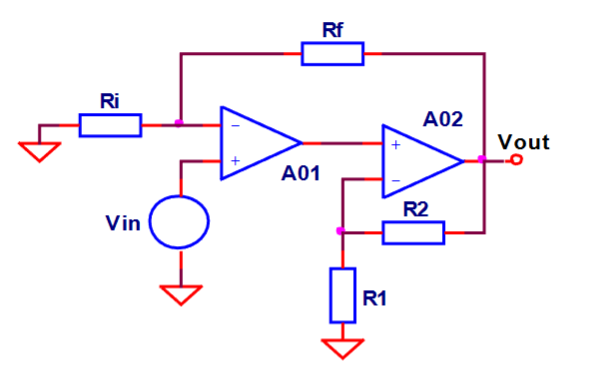
\includegraphics[width=0.5\linewidth]{Imagenes/circuito_1.png}
    \caption{Circuito 1: Amplificador compuesto}
    \label{fig:circuito_1}
\end{figure}

Para este circuito se busca un diseño que obtenga una \textbf{ganancia global} ($A_{vf}$) de 20 dB, compensándolo para obtener una \textbf{máxima planicidad de módulo}, es decir, un margen de fase ($M_\varphi$) de \ang{65} o, equivalentemente, un factor de calidad de los polos ($Q_p$) de $0{,}707$.

\subsection{Caso 1: VFA-VFA}
Como primer caso de estudio se propone utilizar dos amplificadores operacionales de la misma tipología (VFA-VFA) donde se busca:

\begin{enumerate}
    \item Diseñar el amplificador compuesto VFA+VFA
    \item Calcular el ancho de banda potencial.
    \item Determinar la frecuencia del polo de la función de transferencia a lazo cerrado.
    \item Determinar el ancho de banda real a -3dB.
    \item Medir el ancho de banda real
    \item Estimar el margen de fase obtenido en base a la respuesta al escalón.
\end{enumerate}

\subsection{Caso 2: VFA-CFA}
Como segundo caso se busca un circuito que combina las topologías VFA y CFA donde se busca:

\begin{enumerate}
    \item Diseñar el amplificador VFA-CFA para máxima planicidad de módulo y que además cumpla con el ancho de banda potencial aproximado de $f_g = 2\ MHz$
    \item Calcular el ancho de banda potencial
    \item Calcular la frecuencia del polo de la función de transferencia a lazo cerrado
    \item Calcular el ancho de banda real
    \item Medir el ancho de banda a 3 dB.
    \item Estimar el margen de fase obtenido en base a la respuesta al escalón.
\end{enumerate}

\subsection{Caso 3: VFA-CFA (Compensado)}
Como último caso se agrega una red de compensación \textbf{cero - polo} a la salida del VFA al circuito del caso 2. Se busca cancelar el segundo polo del VFA con el cero de la red de compensación y ubicar el polo de la misma por lo menos una octava después para no influir en el mismo. Se busca:

\begin{enumerate}
    \item Retocar la ganancia del CFA para contrarrestar la atenuación producida por la red de compensación.
    \item Calcular el ancho de banda potencial
    \item Calcular la frecuencia del polo de la función de transferencia a lazo cerrado
    \item Calcular el ancho de banda real
    \item Medir el ancho de banda a 3 dB.
    \item Constatar la mejora del margen de fase obtenido en base a la respuesta al escalón.
\end{enumerate}


